\documentclass[12pt,a4paper,twoside]{book}

% use Libertine font
\usepackage{libertine}
\usepackage{inconsolata}
\usepackage[T1]{fontenc}

\usepackage[utf8]{inputenc}
\usepackage[inline]{enumitem}
\usepackage{parskip} % disable indentation for new paragraphs, increased margin-bottom instead
\usepackage[ngerman,american]{babel}
\usepackage{csquotes}

\usepackage{kit_style/kitthesiscover}

\usepackage[style=alphabetic,backend=biber]{biblatex}
\addbibresource{bib.bib}
\addbibresource{bib_manual.bib}
\setcounter{biburlnumpenalty}{100}
\setcounter{biburllcpenalty}{7000}
\setcounter{biburlucpenalty}{8000}

\usepackage{todonotes}
\usepackage{blindtext}

\usepackage{xparse}

\usepackage{xspace}

\usepackage{listings}

% for core allocation pseudo-code mostly...
\usepackage{amsmath}
\usepackage{algorithmicx}
\usepackage{varwidth}
\usepackage{calc} % for \widthof
%\usepackage{algorithm}
\usepackage{algpseudocode}
\usepackage{mathtools}
\DeclarePairedDelimiter\ceil{\lceil}{\rceil}
\DeclarePairedDelimiter\floor{\lfloor}{\rfloor}
\usepackage{amsfonts}
\usepackage{setspace}

% pandas to_latex tables look good this way
\usepackage{booktabs}
\usepackage{multirow}

\usepackage{subcaption}

\usepackage{placeins}

\usepackage{hyperref}

\usepackage{siunitx}

% listings style
\lstdefinestyle{figurec}{
  belowcaptionskip=1\baselineskip,
  language=C,
  basicstyle=\footnotesize\ttfamily,
  frame=single,
  xleftmargin=\parindent,
  alsodigit={:},
}
\lstset{style=figurec}


% custom commands
\newcommand{\impl}[0]{$\Rightarrow$}

\widowpenalty100000
\clubpenalty100000
\raggedbottom

\begin{document}
\frontmatter
\unitlength1cm
\selectlanguage{american}

\title{Low-Latency Synchronous I/O For OpenZFS Using Persistent Memory}
\author{Christian Schwarz}
\thesistype{ma}
\primaryreviewer{Prof.\ Dr.\ Frank Bellosa}
\advisor{M.\ Sc.\ Lukas Werling}{}
\thesisbegindate{TODO}
\thesisenddate{TODO}
\maketitle

\thispagestyle{empty}
\vspace*{30\baselineskip}
%\hbox to \textwidth{\hrulefill}
\par
\iflanguage{ngerman}{
\noindent Ich versichere wahrheitsgem"a"s, die Arbeit selbstst"andig verfasst, alle benutzten Hilfsmittel vollst"andig und genau angegeben und alles kenntlich gemacht zu haben, was aus Arbeiten anderer unver"andert oder mit Ab"anderungen entnommen wurde sowie die Satzung des KIT zur Sicherung guter wissenschaftlicher Praxis in der jeweils g"ultigen Fassung beachtet zu haben.\\

\noindent Karlsruhe, den \declaration@date
}{
\noindent I hereby declare that the work presented in this thesis is entirely my own and that I did not use any source or auxiliary means other than these referenced. This thesis was carried out in accordance with the Rules for Safeguarding Good Scientific Practice at Karlsruhe Institute of Technology (KIT).\\

\noindent Karlsruhe, \declaration@date
}

%%%%%%%%%%%%%%%%%%%%%%%%%%%%%%%%%%%%%%%%%%%%%%%%%%%%%%%%%%%%%%%%%%%%%%%%
%% Hinweis:
%%
%% Diese Erklärung wird von der Prüfungsordnung für Diplomarbeiten 
%% verlangt und ist zu unterschreiben. Für Studienarbeiten ist diese
%% Erklärung nicht zwingend notwendig, schadet aber auch nicht.
%%%%%%%%%%%%%%%%%%%%%%%%%%%%%%%%%%%%%%%%%%%%%%%%%%%%%%%%%%%%%%%%%%%%%%%%
\clearpage








\chapter{Abstract}
\blindtext

\mainmatter
\cleardoublepage
\phantomsection
\addcontentsline{toc}{chapter}{Contents}
\tableofcontents

\chapter{Introduction}
The task of a filesystem is to provide non-volatile storage to applications in the form of the \textit{file} abstraction.
Applications modify files through system calls such as \lstinline{write()} which generally does not provide any durability guarantees.
Instead, the system call modifies a buffer in DRAM such as a page in the Linux page cache and returns to userspace.
Synchronization of the dirty in-DRAM data to persistent storage is thus deferred to a --- generally implementation-defined --- point in the future.

However, many applications have more specific durability requirements.
For example, an accounting system that processes a purchase needs to ensure that the updated account balance is persisted to non-volatile storage before clearing the transaction.
Otherwise, a system crash and recovery after clearing could result in the pre-purchase balance being restored, enabling double-spending by the account holder.
These \textbf{synchronous I/O} semantics must be requested through APIs auch as \lstinline{fsync()} which "assure that after a system crash [...] all data up to the time of the \lstinline{fsync()} call is recorded on the disk."~\cite{posix_fsync_opengroup}.

The \textbf{Zettabyte File System (ZFS)} is a combined volume manager and filesystem.
It pools many block devices into a single storage pool (\textit{zpool}) which can hold thousands of sparsely allocated filesystems.
The ZFS on-disk format is a merkle tree that is rooted in the \textit{uberblock} which is ZFS's equivalent of a superblock.
ZFS on-disk state is always consistent and moves forward in so-called \textit{transaction groups} (txg), using copy-on-write to apply updates.
Whenever a new version of the on-disk state needs to be synced to disk, ZFS traverses its logical structure bottom up and builds a new merkle tree.
The updated parts of the tree are stored in newly allocated disk blocks while unmodified parts are re-use the existing block written in a prior txg.
Once all updates have been written out, the new uberblock is written, thereby atomically moving the on-disk format to its new state.
This procedure is called \textit{txg sync} and is triggered periodically (default: every \SI{5}{s}) or if the amount of dirty data exceeds a configurable threshold.

Synchronous I/O semantics cannot be reasonably implemented through txg sync due to the write amplification and CPU overhead inherent to the txg sync procedure.
Instead ZFS maintains the \textbf{ZFS Intent Log (ZIL)} which is a per-filesystem write-ahead log.
Unlike systems such as Linux's \textit{journaling block device 2} (JBD2), the ZIL is a logical log:
the ZIL's records describe the \textit{logical} changes that need to applied in order to achieve the state that was reported committed to userspace.
On disk, the log records are written into a chain of \textit{log-write blocks} (LWBs), each containing many records.
The LWB chain is rooted in the \textit{ZIL header} within the filesystem's representation within the merkle tree.
New LWBs are appended to the chain independently of txg sync.

By default, LWBs are allocated on\todo{from?} the zpool's main storage devices.
Consequently, the lower bound for synchronous I/O latency in ZFS is the time required to write the LWBs that contains the synchronous I/O operation's ZIL records.
For the case where this latency is insufficient, ZFS provides the ability to add a \textit{separate log device} (SLOG) to the zpool.
The SLOG is typically a single (or mirrored) block device that provides lower latency than the main pool's devices.
A typical configuration today is to add a fast NVMe drive to an HDD-based pool.
Adding a fast SLOG accelerates LWB writes because LWBs are preferentially allocated from the SLOG.
Note that SLOGs only need very limited capacity since LWBs are generally obsolete after three txgs.

\textbf{Persistent Memory (PMEM)} is an emerging storage technology that provides low-latency memory-mapped byte-addressable persistent storage.
The Linux kernel can expose PMEM as a pseudo block device whose sectors map directly to the PMEM space.
Thereby existing block devices consumers can benefit from PMEM' low latency without modification.
Block device consumers that wish to bypass block device emulation use the kernel-internal \textit{DAX} API which translates sector numbers to kernel virtual addresses, giving software \textbf{d}irect \textbf{ac}cess to PMEM.

The motivation for this thesis is to accelerate synchronous I/O in ZFS by using PMEM as a ZFS SLOG device.
A single DIMM of the current\todo{product name} Intel Optane PMEM product line can sustain 530k random 4k write IOPS which corresponds to a write latency of \SI{1.88}{us}.
However, when configuring the Linux PMEM block device as a SLOG in OpenZFS 2.0, a single thread only achieves 12k random 4k synchronous write IOPS~($\sim$~\SI{83}{us}), scaling up to 100k IOPS at 16 threads (8 cores, 2xSMT) at doubled latency.
In contrast, the same workload applied directly to the PMEM block device is able to achieve 500k IOPS with two threads~($\sim$~\SI{4}{us} per thread).
And Linux 5.9's ext4 on the PMEM block device achieves 100k random 4k write IOPS ($\sim$~\SI{}) with a single thread and scales approximately linearly to up to 466k IOPS at four threads.
\todo{review numbers in this paragraph}

Our investigation of the latency distribution for the OpenZFS PMEM SLOG configuration shows that the ZIL implementation contributes \SI{48}{us} in the single-threaded case and up to \SI{95}{us} at eight threads.
More specifically, up to \SI{50}{\%}\todo{run this again without ebpf} of total syscall latency is spent waiting for the \textit{ZIO pipeline}, excluding the time spent in the PMEM block device driver.

ZIO is ZFS's abstraction for performing IO to the pool's storage devices.
The pipeline-oriented design has proven extremely flexible and extensible over ZFS's lifetime.
Many of ZFS’s distinguishing features are implemented in ZIO, including physical block allocation, transparent data and metadata checksumming, compression, deduplication and encryption as well as redundancy mechanisms such as raidz.
CPU-intensive processing steps are parallelized to all of the system's CPUs using \textit{taskq}s.

It is our impression that ZIO is biased towards throughput, not latency.
For example, ZIO's main consumer is \textit{txg sync} which issues the updates to the on-disk merkle tree as a large tree of dependent ZIOs.
Other consumers such as periodic data integrity checking (\textit{scrubbing}) are also throughput-oriented.
In contrast, the ZIL is the only component that is latency-oriented.
ZIO's latency overhead with fast block devices such as NVMe drives is a well known problem among ZFS developers.\todo{ref, gh issue, cite private conversation with brian?}

Given
\begin{itemize}[noitemsep]
    \item the abysmal\todo{too harsh?} out-of-the-box performance of the PMEM block device as a SLOG, and
    \item our findings on\todo{right prep?} the ZIL's and ZIO pipeline's significant latency overhead, as well as the fact that
    \item grouping log records into log-write \textit{blocks} is unnecessary with byte-addressable PMEM,
\end{itemize}
we believe that the current ZIL design is fundamentally unfit to reap the performance available with PMEM.
We present \textbf{ZIL-PMEM}, a new implementation of the ZIL that bypasses the ZIO pipeline completely and persists log entries directly to PMEM.
It coexists with the existing ZIL which we refer to as \textit{ZIL-LWB} in the remainder of this document.
ZIL-PMEM achieves 140k random 4k sync write IOPS with a single thread~($\sim$~\SI{7.1}{us}) and scales up to 400k IOPS at 8 threads before it becomes CPU-bound.
This corresponds to a speedup of 6.8x (or 4x, respectively) over ZIL-LWB.\todo{review numbers}
Our implementation is extensively unit-tested and passes the ZFS test suite's SLOG integration tests.

The remainder of this thesis is structured as follows:
in Chapter 2\todo{automatic chapter numbers} we
review prior work in the field of persistent memory related to filesystems and
provide background knowledge on the integration of PMEM in the Linux kernel as well as
a detailed introduction to the components of ZFS that are relevant for this thesis.
Chapter 3 contains our performance analysis of ZIL-LWB with a PMEM SLOG, making the case for a PMEM-specific ZIL implementation.
The design and implementation of ZIL-PMEM is then presented in Chapter 4, followed by its evalation in Chapter 5.
We conclude with a summary of our findings in Chapter 6.

%In the following sections, we present
%the user experience of configuring a pool with ZIL-PMEM,
%our strategy for code-sharing between ZIL-PMEM and ZIL-LWB and
%the design of ZIL-PMEM, including
%our strategy for how we integrate PMEM log VDEVs into the vdev / zpool config layer
%ZIL-PMEM’s physical data structure,FEe
%its insertion and garbage collection algorithm,
%its claiming & replay algorithm and
%its integration into the existing OpenZFS software architecture.

\chapter{Literature Review \& Background}
In this chapter we present prior work in the field of persistent memory and its application in various storage systems developed in research and industry.
The last two sections on PMEM in Linux and ZFS provide the technical background knowledge that is necessary to understand the performance analysis of ZIL-LWB in Chapter~\ref{ch:lwb_analysis} and the design of ZIL-PMEM in Chapter~\ref{ch:di}.

\section{Literature Review}
We have surveyed publications in the area of persistent memory storage systems, filesystem guarantees \& crash-consistency models, PMEM-specific crash-consistency checkers and general methods to determine filesystem robustness in the presence of hardware failures.

\subsection{PMEM Filesystems}
In this subsection we present research filesystems that were explicitly designed for persistent memory.
ZIL-PMEM integrates into ZFS, a production filesystem that was not designed for persistent memory.
Hence we focus on techniques for crash consistency and data integrity that might be applicable to our work.

\subsubsection{In-Kernel PMEM Filesystems}\label{sec:in_kernel_pmem_filesystems}
The initial wave of publications around the use of PMEM in filesystems produced a set of systems that were implemented completely in the kernel.
\todo{we don't yet compare these systems with ZIL-PMEM. should we? Maybe in a compact section after we presented the design?}

\newcommand{\citerelwork}[2]{\textbf{#1~\cite{#2}}}

\citerelwork{BPFS}{conditBetterByteaddressablePersistent2009} is one of the earliest filesystems expressly designed for PMEM.
The filesystem layout in PMEM is inspired by WAFL~(\cite{hitzFileSystemDesign1994}) and resembles a tree of multi-level indirect pages that eventually point to data pages.
BPFS’s key contribution is the use of fine-grained atomic updates in lieu of journaling for crash consistency.
For example, updates to small metadata such as \textit{mtime} can be made using atomic operations.
For larger modifications, the authors introduce \textit{short-circuit shadow-paging}, a technique where updates are prepared in a copy of the page.
The updated page is then made visible through an update of the pointer in its parent indirect page.
The difference to regular copy-on-write is that, as soon as the update to an indirect page can be done through an atomic in-place operation, the atomic operation is used.
Updates thereby do not necessarily propagatate up to the root of the tree.

\citerelwork{PMFS}{dulloorSystemSoftwarePersistent2014} is another research filesystem that targets persistent memory.
The authors make frequent comparisons to BPFS.
The main differentiator from BPFS with regards to consistency is PMFS’s use of undo-logging for metadata updates and copy-on-write for data consistency in addition to hardware-provided atomic in-place updates.
The evaluation shows that their approach for metadata has between 24x and 38x lower overhead compared to BPFS (unit: number of bytes copied).
PMFS also introduces an efficient protection mechanism against accidental \textit{scribbles}.
Scribbles are bugs in the system that accidentally overwrite PMEM, e.g., due to incorrect address calculation or out-of-bounds access in the kernel.
By default, PMFS maps all PMEM read-only, thereby preventing accidental corruption of PMEM from code outside of PMFS.
When PMFS needs to modify PMEM, it temporarily disables interrupts and clears the processor's \lstinline{CR0.WP}, thereby allowing writes to read-only pages in kernel mode.~\cite{dulloorSystemSoftwarePersistent2014,intelSdmCr0WpFlag}

\citerelwork{NOVA}{xuNOVALogstructuredFile2016} is the most mature research PMEM filesystem.
NOVA uses per-inode logs for operations scoped to a single inode (e.g. write syscalls) and per-CPU journals for operations that affect multiple inodes.
The intended result is high scalability with regard to core count.
The per-inode log data structure is a linked list with a head and tail pointer in the inode.
NOVA leverages 8-byte atomic operations to update these pointers after it has written log entries.
While not explicitly called so by the authors it is our impression that the log is a logical redo log except for writes, which --- judging from the text --- are always logged at page granularity.
The authors explain the recovery procedure and measure its performance but do not address correctness in the evaluation.

\citerelwork{NOVA-Fortis}{xuNOVAFortisFaulttolerantNonvolatile2017} is a version of NOVA that introduces snapshots and hardening against data corruption.
Whereas snapshots are not relevant for this thesis because ZFS already provides this feature, the data corruption countermeasures are representative of the state of the art:
\begin{itemize}[noitemsep,beginpenalty=100000,midpenalty=100000]
    \item Handling of machine check exceptions (MCE) in case the hardware detects bit errors.
          This is done by using \lstinline{memcpy_mcsafe()} for all PMEM access.\todo{ref mcsafe explainer}
          %PMEM data is always buffered in DRAM before it is read.
    \item Detection of metadata corruption through CRC32 checksums.
    \item Redundancy through metadata replication. For metadata recovery, NOVA-Fortis compares checksums of the primary and replica and restores the variant with the matching checksum.
    \item Protection against localized unrecoverable data loss through RAID4-like parity.
          This feature only works while the file is not DAX-mmapped.
    \item Protection against Scribbles using \lstinline{CR0.WP} as described in the paragraph on PMFS.
\end{itemize}
The authors use a custom fault injection tool to corrupt data structures in a targeted manner and test NOVA Fortis's recovery capabilities.

\subsubsection{Hybrid PMEM filesystems}\label{sec:hybrid_pmem_file_systems}
A recurring pattern in PMEM filesystem design is to split responsibilities between kernel and userspace component in order to eliminate system call overhead.

\citerelwork{Aerie}{volosAerieFlexibleFilesystem2014} is a user-space filesystem based on the premise that
“SCM [Storage Class Memory] no longer requires the OS kernel [...].
Applications link to a file-system library that provides local access to data and communicates with a [user-space] service for coordination.
The OS kernel provides only coarse grained allocation and protection, and most functionality is distributed to client programs.
For read-only workloads, applications can access data and metadata through memory with calls to the file-system service only for coarse-grained synchronization.
When writing data, applications can modify data directly but must contact the file-system service to update metadata.”
The system uses a redo log maintained in each client program which is shipped to the filesystem service periodically or when a global lock is released.
It is our understanding that only log entries shipped to and validated by the filesystem service will be replayed.
The authors state that log entries can be lost if a client crashes before the log entries are shipped.
The evaluation does not address crash consistency or recovery at all.

\citerelwork{Strata}{kwonStrataCrossMedia2017} is a cross-media filesystem with both kernel and user-space components.
Since its distinguishing feature is the intelligent migration of data between different storage media we discuss it in the Section~\ref{sec:cross_media_storage_systems} on cross-media storage systems.

\citerelwork{SplitFS}{kadekodiSplitFSReducingSoftware2019} is a research filesystem that proposes a
“split of responsibilities between a user-space library file system and an existing kernel PM file system.
The user-space library file system handles data operations by intercepting POSIX calls, memory-mapping the underlying file, and serving the read and overwrites using processor loads and stores.
Metadata operations are handled by the kernel PM file system (ext4 DAX)”.
SplitFS uses a redo log with idempotent entries that is written from userspace.
As a performance optimization the authors use checksums and aligned start addresses to find valid log entries instead of an explicit linked list with persistent pointers.
The SplitFS evaluation of correctness is limited to a comparison of user-observable filesystem state between SplitFS and ext4 in DAX mode.
Recovery is evaluated only through the lens of recovery time (performance), not correctness.

\citerelwork{EvFS}{yoshimuraEvFSUserlevelEventDriven2019} is a
“user-level POSIX file system that directly manages NVM in user applications.
EvFS minimizes the latency by building a user-level storage stack and introducing asynchronous processing of complex file I/O with page cache and direct I/O.
[...]
EvFS leads to a 700-ns latency for 64-byte non-blocking file writes and reduces the latency for 4-Kbyte blocking file I/O by 20 us compared to a kernel file system [EXT4] with journaling disabled.“
In contrast to Aerie, EvFS does not require a coordinating user-space service.
Crash consistency and recovery is not addressed:
“EvFS is not a production-ready file system because it neither provides all the POSIX APIs or crash-safe properties”.

\subsection{Cross-Media Systems}\label{sec:cross_media_storage_systems}
Cross-media storage systems combine the advantages of multiple storage devices from different levels of the storage hierarchy.
Historically, these kinds of systems strive to exploit hard disk for high capacity at low cost and more expensive flash storage for low latency random access IO.
With persistent memory, a new class of storage has become available whose role in cross-media systems is still to be determined.
In the context of this thesis we find it most useful to compare the overall system architecture.

\citerelwork{ZFS: Allocation Classes}{openzfsAllocationClasses}
Whereas ZFS was initially designed for a large pool of hard disks, it has gained several cross-media features over its lifetime.
When configuring a zpool, the administrator assigns the block device to an \textit{allocation class}.
The following allocation classes exist: \textit{normal} (main pool), \textit{log} (SLOG device), \textit{aux} (L2ARC, a victim cache for ZFS's ARC\todo{check that we have explained ARC already}), \textit{special} (small blocks), and \textit{dedup} (deduplication table data).
When a function in ZFS allocates a block in the pool, it must specify the desired allocation class.
If the allocation succeeds, the allocated block is guaranteed to be located on device(s) within that class.
The use case for allocation classes is to combine the advantages of different storage media in a single pool.
In many setups devices in the \textit{normal} class have high capacity and are grouped in storage-efficient redundancy configurations such as \textit{raidz} or \textit{draid}.
A \textit{log} or \textit{aux} device can be added to a pool in order to accelerate latency-sensitive I/O such as ZIL writes.
Many administrators configure lower redundancy for these devices --- either to gain performance or to reduce costs --- which, depending on business requirements, may be justified due to the short-lived nature of ZIL writes.
In comparison to the other systems presented in this section, allocation classes are very inflexible:
once an allocation is made and the data is written, the data stays in that place until it is freed or the device is removed from the pool.
In particular, there is no automatic tiering that takes usage patterns into account.
Further, L2ARC devices reduce space efficiency because the cached data still occupies space in the main pool.
Similarly, SLOG devices are somewhat wasteful since they are exclusively used for ZIL logging and never read except during recovery.
Systems such as Strata derives more value from its PMEM-based log.
Finally, it should be noted that while Linux's /dev/pmem\todo{ref backwards} block device can be used with allocation classes, ZFS's ZIO pipeline is unable to exploit its write performance.\todo{ref section on ZIL-LWB perf}.
%On the write path, separate log devices (SLOG) can be added to a storage pool to be used exclusively for persisting ZFS’s logical write-ahead log (the ZIL).
%Offloading latency-sensitive IO to the log device allows for greater throughput during txg sync to the main pool’s devices.
%\todo{if we move the related work section to the end of the thesis this paragraph can be abbreviated}
%On the read path, the in-DRAM ARC, which is ZFS’s variant of the buffer cache, can be extended with a second-level victim cache on a block device, the L2ARC.
%L2ARC hits free up IOPS among the main pool’s devices which can be used for txg sync.

\citerelwork{ZFS: ZIL Performance Improvements For Fast Media}{openzfsZILPerformanceImprovements2020}
At the OpenZFS 2020 Developer summit, Saji Nair of storage vendor Nutanix presented a ZIL prototype that handles fast block devices more efficiently.
The prototype avoids unnecessary sequential ordering of I/O operations when writing ZIL LWBs\todo{check that LWBs have been introduced by now}.
It also avoids using the ZIO pipeline due to context switching overheads, issuing block I/O directly from the application thread instead.
The evaluation is limited to 4k sync write performance, claiming an up 4x improvement in IOPS with four threads.
However, the source code for the prototype has not been published and the design is incomplete with regards to replay.
\todo{maybe this entire section should move to the 'background' section?}

\citerelwork{Strata}{kwonStrataCrossMedia2017} is a cross-media research filesystem.
“Closest to the application, Strata’s user library synchronously logs process-private updates in NVM while reading from shared, read-optimized, kernel-maintained data and metadata.
    [...]
Client code uses the POSIX API, but Strata’s synchronous updates obviate the need for any sync-related system calls”.
We classify Strata as a hybrid filesystem in Section~\ref{sec:hybrid_pmem_file_systems} because it consists of both a userspace library and an in-kernel component.
The log, written from userspace, is an idempotent logical redo log.
The kernel component then \textit{digests} the logs asynchronously, performing aggregation of the logged operations during digestion.
Aggregation permits the kernel component to issue “sequential, aligned writes” to the slower storage devices such as SSDs or HDDs.
ZFS with and without ZIL-PMEM compares to Strata in the following ways:
\begin{itemize}[noitemsep,beginpenalty=100000,midpenalty=100000]
    \item Both systems use a logical redo operation log instead of a block-level journaling mechanism.
    \item Both systems perform asynchronous write-back and thereby reap similar benefits from it (parallel batch processing, optimized allocation).
    \item Strata’s kernel component digests the logs written from user-space in order to write them back to other tiers.
          ZFS accumulates the write-back state in DRAM and never reads the log except for recovery.
          (It is unclear to us how often Strata digests the logs. ZFS performs write-back of dirty state after at most 5 seconds.)
          % \item The Strata paper suggests that the system uses a single block size whereas ZFS supports variable block sizes (“Free Block Bitmap” in Strata vs. Spacemaps in ZFS).
    \item Strata seems to tune allocations for SSDs, e.g. allocating blocks in erasure block size to prevent write amplification.
          ZFS supports TRIM and supports variable block sizes up to \SI{16}{MiB}, but there are no automatic optimizations that specifically target write amplification in SSDs.
          %\item ZFS guarantees data integrity and has provisions for redundancy.
          %\item ZFS supports many devices at different performance class levels whereas Strata only supports a single device.
    \item ZFS is in-kernel and requires no modifications to applications whereas Strata requires linking to or LD\_PRELOADing a user-space library, which, tangentially, makes it incompatible with statically linked binaries.
          %\item ZFS is a mature filesystem used at large scale in production whereas Strata is an unproven research prototype.
\end{itemize}

\citerelwork{Ziggurat}{zhengZigguratTieredFile2019}
“Ziggurat exploits the benefits of NVMM through intelligent data placement during file writes and data migration.
Ziggurat includes two placement predictors that analyze the file write sequences and predict whether the incoming writes are both large and stable, and whether updates to the file are likely to be synchronous.
Ziggurat then steers the incoming writes to the most suitable tier based on the prediction: writes to synchronously-updated files go to the NVMM tier to minimize the synchronization overhead.
Small, random writes also go to the NVMM tier to fully avoid random writes to disk. The remaining large sequential writes to asynchronously-updated files go to disk”.
The authors compare Ziggurat to Strata as follows:
“Strata is a multi-tiered user-space file system that exploits NVMM as the high-performance tier, and SSD/HDD as the lower tiers.
It uses the byte-addressability of NVMM to coalesce logs and migrate them to lower tiers to minimize write amplification.
File data can only be allocated in NVMM in Strata, and they can be migrated only from a faster tier to a slower one.
The profiling granularity of Strata is a page, which increases the bookkeeping overhead and wastes the locality information of file accesses".
ZFS with and without ZIL-PMEM compares to Ziggurat as follows:
\begin{itemize}[noitemsep,beginpenalty=100000,midpenalty=100000]
    \item Ziggurat actively migrates data into PMEM based on access pattern.
          ZFS has no provisions for data migration within the pool after block allocation.
          The ZFS architecture such a feature is unlikely to be developed in the future (keyword: blockpointer rewrite).
    \item Ziggurat sends writes directly to the suitable tier based on prediction of future access patterns.
          If the access pattern is anticipated to be synchronous, Ziggurat choses the PMEM tier.
          The ZIL, and ZIL-PMEM specifically, only serves as a stop-gap between txg sync points of the main pool.
          Data is always written twice --- once to the log and once to the main pool ---, and never read from the log except during recovery.
          %(The \lstinline{WR_INDIRECT ZIL} log entry type mitigates this for large writes).
    \item Both systems are fully in-kernel and require no modifications to user-space applications.
    \item Ziggurat builds on NOVA-Fortis and thus inherits the PMEM-specific data integrity and redundancy mechanisms provided for the PMEM storage tier.
          ZIL-PMEM data integrity measures are more limited but can be expanded in the future (see Chapter~\ref{ch:di}).
    \item The Ziggurat paper does not mention data integrity measures or redundancy mechanisms for the block device layers beneath PMEM.
          Possibly, existing Linux features such as Device Mapper could be used to compensate.
          In contrast, ZIL-PMEM benefits from ZFS’s strong data integrity and redundancy mechanisms once the logged data is txg synced.\todo{ensure txg sync has already been explained}
    \item The Ziggurat design is “fast-first. It should use disks to expand the capacity of NVMM rather than using NVMM to improve the performance of disks as some previous systems have done”.
          ZIL-PMEM approaches persistent memory from the opposite direction, starting with a filesystem strongly focussed on block devices and only leveraging PMEM where appropriate.
    \item Ziggurat was not evaluated on actual persistent memory. The authors used memory on another NUMA node to simulate lower latencies.
          We evaluate ZIL-PMEM on commercially available PMEM hardware.
          %\item An examination of the Ziggurat code base shows that it only supports a single device per tier.
          %\item Ziggurat has been unmaintained since the publication. OpenZFS has a healthy community of both hobbyist and paid full-time contributors.
\end{itemize}

\citerelwork{dm-writecache}{WritecacheTargetLinux} is a new Linux Device Mapper target that synchronously persists writes to PMEM and performs asynchronous writes-back to the origin block device in the background.
Dm-writecache is relevant to ZIL-PMEM because both systems expose a PMEM-accelerated virtual block device.
For this use case, a write-back cache can be more space efficient because it only needs to store the most recent version of a block.
In contrast, ZIL-PMEM logs each block write (smallest block size for ZVOLs is 4k) separately and does not coalesce or delta-encode log entries.
ZIL-PMEM protects data integrity through checksums whereas dm-writecache fully relies on hardware error correction and detection, reported via \lstinline{memcpy_mcsafe()}.
Once ZVOL modifications are txg-synced\todo{backref} to the main pool, they benefit from ZFS's strong data redundancy mechanisms such as \textit{raidz}.
With dm-writecache, the origin block device driver must handle data redundancy if desired, e.g., though another Device Mapper target such as \textit{dm-raid}.
We compare the performance of the two implementations in Section X.Y \todo{ref block device comparison}):
dm-writecache delivers on the promise of low latency but shows significant lock contention with multiple threads, failing to saturate PMEM bandwidth and performing significantly worse than ZIL-PMEM.\todo{verify claim}

\subsection{Journaling \& Write-Ahead Logs Adapted PMEM}
The following publications use persistent memory to accelerate file system journals and write-ahead logs.

\citerelwork{Unioning of the Buffer Cache and Journaling Layers with Non-volatile Memory}{leeUnioningBufferCache2013} is an academic paper that presents a PMEM-aware buffer cache design which
“subsumes the functionality of caching and [block-level] journaling”.
From the buffer cache’s perspective, the on-disk blocks that make up a journal (e.g. one managed by JBD2) are indistinguishable from non-journal filesystem blocks.
Thus, for a journal block $A’$ that logs an update to a block $A$, both blocks $A’$ and $A$ will sit in the buffer cache.
This waste of space can be reduced with PMEM by the author’s proposal.
Instead of journaling on top of the block layer, one journals in the buffer cache itself by a) placing the buffer cache in PMEM and b) introducing a new buffer cache entry state “frozen” so that an entry can be “clean”, “dirty” or “frozen”.
When modifying a block $A$, the filesystem no longer makes a journal entry but instead modifies the buffer cache entry directly.
If the entry was “clean”, it is now “dirty”. If the entry was “frozen”, a copy is made and the modification goes to the copy, making it “dirty” as well.
Committing a block to the journal is a simple state transition from “dirty” to “frozen”. On a crash + restart, “dirty” buffer cache entries are discarded but “frozen” entries remain.
We find the approach exceptionally interesting and innovative and can imagine an application of the idea to the ZFS ARC.
However, the system’s real-world performance is unclear (evaluation on DRAM).
Also, we see non-trivial software engineering and maintenance problems with the approach.
Finally, the paper does not address hardware error handling or data corruption concerns at all.

\citerelwork{ext4 fast commits}{FastCommitsExt4} is a feature released in Linux 5.10.
“The fast-commit journal [...] contains changes at the file level, resulting in a more compact format.
Information that can be recreated is left out, as described in the patch posting:
For example, if a new extent is added to an inode, then  corresponding updates to the inode table, the block bitmap, the group descriptor and the superblock can be derived based on just the extent information and the corresponding inode information.
    [...] Fast commits are an addition to — not a replacement of — the standard commit path; the two work together.
If fast commits cannot handle an operation, the filesystem falls back to the standard commit path.”
The cited article mentions ongoing work to use persistent memory for ext4 fast commits.
The approach is inspired by per-inode journaling as proposed by \citeauthor{parkIJournalingFinegrainedJournaling2017} in \cite{parkIJournalingFinegrainedJournaling2017}.

\textbf{Disk-oriented database management systems} often use write-ahead logs (WALs) to allow a transaction to commit before the modified pages are written back to stable storage.
However, appending to a shared WAL file has historically been a latency and scalability bottleneck which lead to amortization techniques such as \textit{commit groups} (aka \textit{group commit}) and \textit{pre-committed transactions} that batch the WAL entries of multiple committing transactions into a single physical WAL record.%
\footnote{According to \cite{dewittImplementationTechniquesMain1984} "the notion of gronp commits appears to be past of the unwritten database folklore. The System-R implementors claim to have implemented it."}
With persistent memory, the latency bottleneck no longer lies in the raw I/O but rather the coordination overhead between multiple CPU cores and sockets, prompting new distributed logging designs that avoid a central point of contention.%
~\cite{fangHighPerformanceDatabase2011,pelleyStorageManagementNVRAM2013,johnsonAetherScalableApproach2010}
ZIL-LWB\todo{ensure this term has been established by now} employs \textit{group commit} as well although the terminology is different.
It batches log records issued by independent threads for the same filesystem into the currently \textit{open} \textit{log-write block} (LWB).
Once the open LWB is full or a timeout has passed, the open LWB is written (\textit{issued}) to disk.\todo{refer to section that explains the perf problems with ZIL-LWB}
In contrast, ZIL-PMEM commits log records directly to PMEM and allows multiple cores to do so in parallel with minimal global coordination.\todo{minimal global coordination = the committer slots + semaphore}
Our evaluation shows that the design scales well on single-socket systems.
NUMA and multi-socket systems, which are addressed in the cited publications from the database community, have been explicitly out of scope for this thesis.\todo{meh, ref}

\subsection{Testing Filesystem Crash Consistency}
In this section we survey techniques to determine and verify crash consistency guarantees of file systems.
A formal and automatically verifiable model would have been been extremely helpful to ensure that ZIL-PMEM maintains the same crash consistency guarantees as ZIL-LWB.\todo{ref}

\citerelwork{All File Systems Are Not Created Equal}{pillaiAllFileSystems2014} contributes a survey of the atomicity and ordering guarantees of several popular Linux filesystems and provides a tool called ALICE to validate or derive the guarantees required by applications.
ZFS with and without ZIL-PMEM could benefit from this survey as well.
The survey could be used to characterize ZFS’s guarantees.
ALICE could be used to determine whether ZFS’s guarantees are sufficient for applications and/or whether ZFS’s guarantees exceed the requirements of the majority of applications.
However, since ZIL-PMEM shall maintain the same guarantees as ZIL-PMEM (see Section~\ref{sec:requirements}), such findings would only be relevant for future work.

\citerelwork{Specifying and Checking File System Crash-Consistency Models}{bornholtSpecifyingCheckingFile2016}
The authors
“present a formal framework for developing crash-consistency models, and a toolkit, called FERRITE, for validating those models against real file system implementations.”
The system provides means to express expected filesystem behavior as a \textit{litmus test}.
A litmus test encodes expected behavior of a filesystem though a series of events (e.g. write to a file) and a final predicate expressed as a satisfiability problem.
FERRITE can execute the litmus test against an axiomatic formal model of the filesystem to ensure that, iff the actual filesystem adheres to the formal model, the litmus test’s expectations hold.
Notably the litmus test is executed symbolically and the validation predicates are checked for satisfiability by an SMT solver; this is exhaustive and not comparable to a unit  or regression test.
FERRITE can also execute litmus tests against the actual filesystem to test whether it adheres to the formal model.
This test is non-exhaustive.
It is based on executing the litmus test “many times” where for each execution all disk commands emitted during execution are recorded.
All permutations and prefixes of these traces that are allowed under the semantics of the disk protocol are used to produce test disk images which are fed back to the filesystem under test for recovery.
After recovery the litmus test’s predicate must hold against the concrete filesystem state after recovery.
If it does not hold the given permutation of the trace is proof that the filesystem does not match its model (assuming the litmus test passes execution against the model), or that the filesystem’s assumptions about the disk do not match the FERRITE \textit{disk model}.
FERRITE appears to be a useful tool to build a model of ZFS’s undocumented crash-consistency guarantees (ZFS has not been evaluated by the authors).
Such a model would be helpful to validate ZIL-PMEM's goal to maintain the same semantics as ZIL-PMEM.
However, this would require a FERRITE disk model for persistent memory.

\citerelwork{Using Model Checking to Find Serious File System Errors}{yangUsingModelChecking2006}
The authors present an “implementation-level model checker” that removes the need to define a formal model for the filesystem.
Instead, the model is inferred by running the OS with the filesystem and recording both syscalls emitted by the application and disk operations emitted by the filesystem.
These traces are subsequently fed to a process that produces disk images created from reorderings of disk operations.
The disk images are fed to the filesystem’s fsck tool.
Disk images that can be ‘repaired’ by fsck are then fed to the “recovery checker” which examines filesystem state and compares it to the expected state which (if we understand section 4.2 of the paper correctly) is derived from the recorded system calls.
(The role of the “volatile file system” in this process is still unclear to us).
The authors mention several shortcomings of their system:
\begin{itemize}[noitemsep,beginpenalty=100000,midpenalty=100000]
    \item Lack of multi-threading support (this applies to FERRITE as well).
    \item The recovery checker produces a projection of the filesystem state (e.g. only names and content but no atime).
          Thus, the system can only check guarantees at the projection level.
    \item Restrictive assumptions such as “Events should also have temporal independence in that creating new files and directories should not harm old files and directories”.
\end{itemize}
The idea of using the filesystem’s recovery tools (fsck) to infer its guarantees seems useful to avoid the requirement of a formally specified model.
However, it is our understanding that the resulting model is rather a larger regression test than a truly derived exhaustive model.
Such regression tests would be useful as a starting point for a formal model, e.g., as initial litmus tests for use with FERRITE.
We do not believe that we can apply the presented approach to ZFS with and without ZIL-PMEM with reasonable effort.

\subsection{PMEM-specific Crash-Consistency Checkers}
A growing body of work introduces tools that check whether code that manipulates persistent memory actually issues the architectually required instructions for persistence.\todo{phrasing is odd?}
However, most systems only target userspace code and are thus inapplicable to ZIL-PMEM which is implemented in the ZFS kernel module.
Whereas ZIL-PMEM can be compiled for user-space as part of the \textit{libzpool} library, the large amount of conditional compilation involved in the libzpool build process diminishes the significance of user space tests.
We surveyed the following userspace-only tools:
\begin{itemize}[noitemsep,beginpenalty=100000,midpenalty=100000]
    \item \citerelwork{pmemcheck}{intoductionToPmemcheckPart}, a tool in Intel’s Persistent Memory Development Kit (PMDK).
          It integrates with Valgrind~(\cite{Valgrind}) and requires annotation of all PMEM accesses.
          Notably, the PMDK libraries include these annotations.
    \item pmeminsp\todo{todo}
    \item Agamotto \todo{todo}
\end{itemize}
The remaining tools in this subsection support kernel code and could be applicable to ZIL-PMEM.

\citerelwork{Yat: A Validation Framework For Persistent Memory Software}{lantzYatValidationFramework2014}
“Yat is a hypervisor-based framework that supports testing of applications that use Persistent Memory [...]
By simulating the characteristics of PM, and integrating an application-specific checker in the framework, Yat enables validation, correctness testing, and debugging of PM software in the presence of power failures and crashes.”
The authors used Yat to validate PMFS (see Section~\ref{sec:in_kernel_pmem_filesystems}).
Yat's hypervisor-based approach makes it the ideal tool for evaluating ZIL-PMEM.
To our great dissatisfaction, Yat has never been published and remains an Intel-internal project.

\citerelwork{PMTest: A Fast And Flexible Testing Framework For Persistent Memory Programs}{liuPmtestFastFlexible2019}
PMTest is a validation tool that claims to be significantly faster than Intel's \textit{pmemcheck}.\todo{we introduced it above, context still there?}
The implementation is based on traces of PMEM operations which are generated by (manually or automatically) instrumented application code.
PMTest ships with two built-in checkers that assert correct instruction ordering (e.g.: missing store barriers) and durability (e.g.: missing cache flushes).
Higher-level checks must be implemented by the programmer.
PMTest works within kernel modules but the implementation is limited to a single thread.
The processing of the operation trace happens in userspace.
PMTest could be used to check ZIL-PMEM kernel code: for a single ZPL filesystem and a single thread that performs synchronous I/O, the pool's PMEM is only written from that thread.\todo{ref design sections}

\subsection{Fault Injection}
Error handling code are notoriously difficult to test but often critical for correctness.
Fault injection is a common technique to simulate failures and thereby exercise these code paths.

\citerelwork{Model-based Failure Analysis Of Journaling File Systems}{prabhakaranModelbasedFailureAnalysis2005}
The authors present an analysis of the failure modes caused by incorrect handling of disk write failures in the journaling code in ext4, ReiserFS and IBM JFS.
These filesystems each implement one or more of the following journaling modes: data journaling, ordered journaling, and writeback journaling.
Any block write performed in one of these modes falls in one of the following categories:
“J represent journal writes, D represent data writes, C represent journal commit writes, S represent journal super block writes, K represent checkpoint data writes [...]”.
For each of the three journaling modes, the authors present a state machine that describes all permitted sequences of block writes.
The state machine includes transitions to an error state if a block write fails.
The system works as follows.
A kernel module tracks the filesystems' state as modelled by the state machine.
It intercepts block device writes from the filesystem code and injects write failures.
If the filesystem subsequently performs another block write that is not permitted by the state machine, an implementation error has been found.
The authors distinguish several classes of failures with varying degrees of data loss.
The methodology is very filesystem specific which already shows in the adjustments required for IBM JFS.
The ZIL's structure and its interaction with txg sync\todo{ref sections} is substantially different from the journaling modes presented in the paper.
The system is thus not applicable to ZIL-PMEM.

\citerelwork{ndctl-inject-error}{NdctlinjecterrorManPage} is a subcommand of the \lstinline{ndctl} administrative tool that
"can be used to ask the platform to simulate media errors in the NVDIMM address space to aid debugging and development of features related to error handling."
The kernel driver forwards injection requests to the NVDIMM firmware via ACPI.~\cite{NdctlPATCHV2}
The errors then surface as \textit{machine check exceptions} (MCE), which is the same mechanism used to indicate detected but uncorrectable ECC errors for DRAM and PMEM.
The functionality is useful for testing correct error in the filesystem when \textit{reading} PMEM.
ZIL-PMEM does not use \lstinline{memcpy_mcsafe()} when accessing persistent memory and therefore does not handle MCEs on read.\todo{can we fix this until submission?}
However, if ZIL-PMEM used \lstinline{memcpy_mcsafe()}, the error handling would be the same as for corrupted or missing log entries, for which we have good unit test coverage.\todo{ref evaluation}

\citerelwork{ZFS Fault Injection}{ZinjectOpenZFSMan}
The ZFS tool \textit{zinject} allows for targeted injection of artifical IO failures.
Errors can be scoped to an entire device or specific logical data objects in ZFS.
The ZFS integration test suite makes use of the command for high-level features such as automatic hot spares.
ZIL-PMEM does not use ZIO to access PMEM and thus cannot hook into the zinject infrastructure.
Most of the semantics are tied to ZFS’s \lstinline{zbookmark} and \lstinline{blkptr} structures which we do not use in ZIL-PMEM.
We expect that proper adaptation of zinject to ZIL-PMEM would be difficult.
A ZIL-PMEM specific tool that allows fault injection or even manipulation of log entries in PMEM would be useful for debugging and integration testing.
However, the existing ZIL-PMEM unit tests already test many scenarios for data corruption in a more expressive and efficient manner.

\section{Persistent Memory in Linux}

%Data corruption, MCE, memcpy_mcsafe
%-> NOVA Fortis paper
%-> https://software.intel.com/content/www/us/en/develop/articles/error-recovery-in-persistent-memory-applications.html
%-> https://software.intel.com/content/www/us/en/develop/articles/pmem-RAS.html
%ent of a \textit{machine check exceptions} (MCE) triggered by a PMEM hardware error.
%The behavior for MCE with PMEM is similar to that with ECC.
%If the MCE happens in userspace\todo{review userspace vs user-space vs user space}, Linux converts it into SIGBUS signals.
%In the kernel, an MCE triggers a panic unless the \lstinline{memcpy_mcsafe()} API is used which returns an error value if an MCE occurred.
%The code that called \lstinline{memcpy_mcsafe()} can thus treat read errors as IO errors.
%The value that \lstinline{memcpy_mcsafe()} provides to ZIL-PMEM is very limited because it only handles read errors.
%ZIL-PMEM does not use could use \lstinline{memcpy_mcsafe()} 
%The value of MCEs and \lstinline{memcpy_mcsafe()} is very limited in the context of ZIL-PMEM because it only reads PMEM during pool import and replay.
%At this point, errors from memcpy_mcsafe() are handled the same way that corrupted log entries are handled.
%A mechanism to handle write failures to PMEM would be very useful
%Also: \cite{PersistentmemoryErrorHandling}
%The problem there is that store operations are not usually synchronous, so there will be no immediate indication of an error. Paranoid software can [Jeff Moyer] do a flush and a load after every store to ensure that the data has been stored properly; there does not seem to be any better way.

\section{OpenZFS Primer}

\subsection{The ZIL API}\label{openzfs:the_zil_api}
The \textit{zil.c} code module implements all ZIL functionality.
The ZIL is a per-dataset log and thus all ZIL state is kept in per-dataset structures.
On disk, this state is kept in the \lstinline{zil_header_t} structure, which is part of the \lstinline{objset_phys_t} structure.
\lstinline{zil_header_t} contains the pointer to the first LWB in the dataset's ZIL chain.
It also contains fields that track claiming and replay progress.
In DRAM, the per-dataset state is kept in the \lstinline{zilog_t} structure.
All ZIL APIs are effectively scoped to the \lstinline{zilog_t}. %either by explicitly taking a pointer to the dataset's \lstinline{zilog_t} as an argument or implicitly by being scoped to a particular dataset
On the write path, the following ZIL APIs are relevant:
\begin{description}
    \item[zil\_itx\_create] Allocate an ITX with a given record size.
    \item[zil\_itx\_assign] Associate the given ITX with the changes made in the given DMU transaction.
          The call moves ownership of the ITX to \lstinline{zilog_t}.
    \item[zil\_commit] Persist previously assigned ITXs to stable storage.
          The caller can specify the object ID of a \lstinline{znode} to inidicate that it is sufficient to persist the ITXs that affect this \lstinline{znode}.
          This functionality enables efficient \lstinline{fsync()} if some files are written asynchronously and some synchronously.
\end{description}
The activity diagrams in Figure~\ref{fig:zil_api_syscall_activity_diagrams} visualize how these APIs are used in \lstinline{write()}, \lstinline{fsync()}, and \lstinline{sync()} system calls.
\begin{figure}[h]
    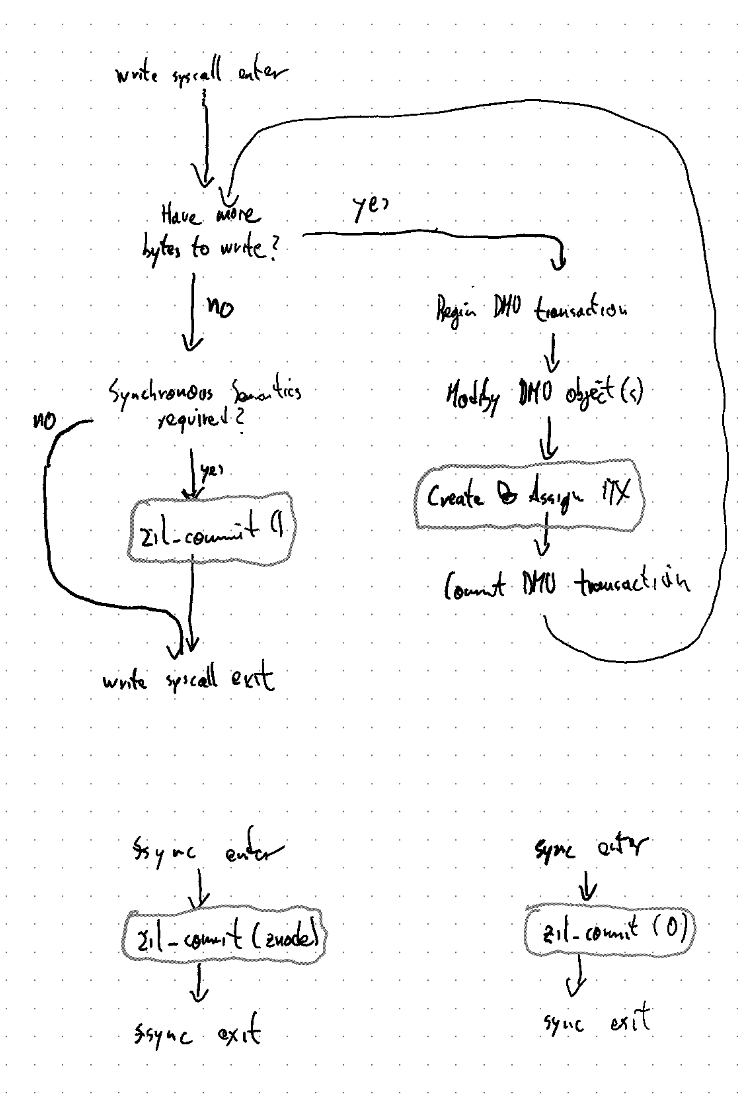
\includegraphics[height=0.8\textheight]{fig/zil_api_syscall_activity_diagrams}
    \caption{
        ZIL API usage on the write path in \lstinline{write()}, \lstinline{fsync()}, and \lstinline{sync()} system calls.
    }
    \label{fig:zil_api_syscall_activity_diagrams}
\end{figure}

\lstinline{zilog_t} tracks assigned ITXs in data structures called \lstinline{itxg}.
There exists one \lstinline{itxg} per unsynced pool transaction group (txg).
When an ITX is assigned to the ZIL in a given txg, it is added to that txg's \lstinline{itxg}.
After the txg sync thread has finished syncing a txg, it frees the corresponding \lstinline{itxg} and all the ITXs in it because the changes they describe are now persisted in the main pool and thus obsolete.

Each \lstinline{itxg} is split into a \textit{sync list} and the \textit{async tree}.
The \textit{sync list} is a simple list of ITXs whereas the \textit{async tree} is a search-tree that maps from object ID to a list of ITXs.
By default, ITXs are added to the \textit{sync list} when assigned to the ZIL.
The \textit{async tree} is only used for ITXs that are scoped to a particular file.
For example, an ITX that logs the creation of a file is added to the \textit{sync list} whereas a write within that file is added to the \textit{async tree}.

\lstinline{zil_commit} uses the \lstinline{itxg}s to build a linear \textit{commit list} of ITXs that it can subsequently persist to stable storage.
The pseudo-code in Figure~\ref{lst:zil_commit} illustrates the construction of the commit list by \lstinline{zil_commit}.
Figure~\ref{fig:zil_per_itxg_state_example} provides an example for a single transaction group.
\begin{figure}[h]
    \begin{lstlisting}
zil_commit(object_id)
    commit_list := []
    for each unsynced transaction group 'txg':
        itxg <- the itxg for txg
        if object_id == 0:
            append all itxs in itxg.async to itxg.sync
        else:
            append only the itxs in
              itxg.async[object_Id] to itxg.sync
        append itxg.sync to commit_list
    err := persist commit_list
    if err:
        wait until the open txg has synced
    return
\end{lstlisting}
    \caption{Pseudo-code that illustrates the work done by \lstinline{zil_commit()}.}
    \label{lst:zil_commit}
\end{figure}

\begin{figure}[h]
    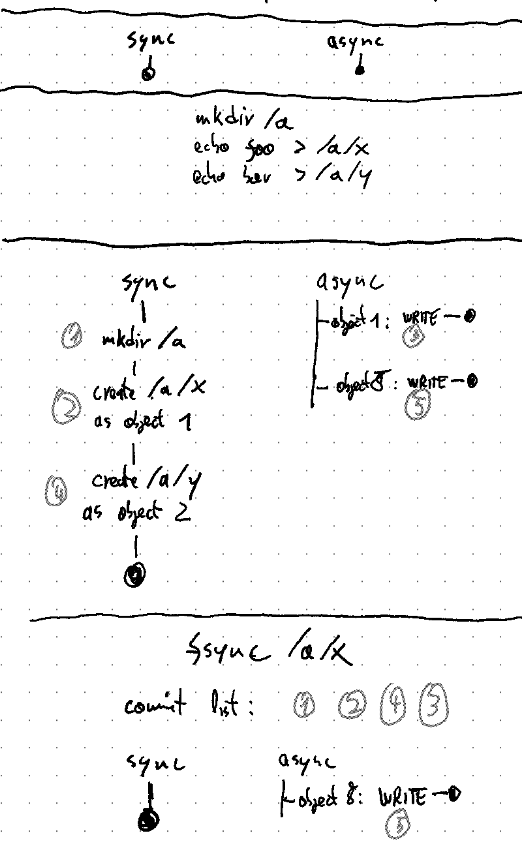
\includegraphics[height=0.5\textheight]{fig/zil_single_itxg_example}
    \caption{
        An example of how an itxg is filled with ITXs and how \lstinline{zil_commit} drains it into a commit list.
        Note that this example only covers the case where all ITXs were assigned for the same txg.
    }
    \label{fig:zil_per_itxg_state_example}
\end{figure}


\chapter{Why ZIL-LWB Is Slow On PMEM}\label{ch:lwb_analysis}
\blindtext\todo{blindtext}

\chapter{Design \& Implementation}
In this chapter we present the design and implementation of ZIL-PMEM in OpenZFS.
We start with an outline of the project goals and limitations, followed by a high-level overview of the design.
Each of the subsequent sections then presents one orthogonal concept in more detail, including implementation aspects where appropriate.
Readers should be familiar with the technical background on PMEM in Linux and OpenZFS given in Section~\todo{ref}.

\section{Project Scope}

\newcommand{\csgoal}[1]{\textbf{#1}}

\subsection{Requirements}\label{sec:requirements}
The following features are success criteria for the ZIL-PMEM design.

\csgoal{Coexistence}
ZIL-PMEM must coexist with ZIL-LWB due to limited availability of PMEM and limitations of the ZIL-PMEM design.

\csgoal{Same Guarantees}
ZIL-PMEM must maintain the same crash consistency guarantees towards user-space as ZIL-LWB for both ZPL and ZVOL.

\csgoal{Simple Administration \& Pooled Storage}
Pooling of storage resources and simple administration are central to ZFS.~\cite{bonwickZettabyteFileSystem2003}
ZFS should automatically detect that a SLOG device is PMEM and, if so, use ZIL-PMEM for all of the pool’s datasets.
No further administrative action should be required to fully benefit from ZIL-PMEM.

\csgoal{Correctness}
In the absence of PMEM media errors and data corruption, ZIL-PMEM must be able to replay all data that it reported as committed.
The result must be the same as if ZIL-LWB would have been used in lieu.
Specifically:
\begin{itemize}[noitemsep,beginpenalty=100000,midpenalty=100000]
    \item Replay must respect the logical dependencies of log entries.
    \item Logging must be crash-consistent, i.e., the in-PMEM state must always be such that replay is correct.
    \item Replay must be crash-consistent, i.e., if the system crashes or loses power replay must be able to resume. Resumed replay must continue to respect logical dependencies of log entries.
\end{itemize}

\csgoal{Data Integrity}
Data integrity is a core feature of ZFS.~\cite{bonwickZettabyteFileSystem2003}
ZIL-PMEM must detect corrupted log entries using an error-detecting code.
Detected corruption must be handled \textit{correctly} as outline in the previous paragraph.
It must also be handled gracefully with the following behavior as the baseline:
"Assume a sequence of log entries $1 \dots N$ where log entry $1$ does not depend on a log entry and each entry $i > 1$ depends on its predecessor $i-1$.
Data corruption in entry $i \in 1 \dots N$ must not prevent replay of entries $1 \dots i-1$".

\csgoal{Low Latency}
The latency overhead of ZIL-PMEM compared to raw PMEM device latency should be minimal for single threaded workloads.
Multi-threaded workloads are addressed below.

\csgoal{Multi-Core Scalability}
Since PMEM is added as a pool-wide resource used by all of the pool's datasets, ZIL-PMEM should scale well to multiple cores.
Barring PMEM throughput limitations, ZIL-PMEM should achieve the following speedups for threads that perform synchronous I/O operations on separate CPU cores:
{
\setlength{\parskip}{0pt}
\begin{description}[topsep=0pt, noitemsep, leftmargin=1cm, labelindent=1cm, widest=1 private dataset per thread]
    \item[1 private dataset per thread] Always near-linear speedup.
    \item[1 shared dataset] \mbox{}
          \begin{description}[noitemsep, leftmargin=1cm, labelindent=1cm, widest=ZPL filesystem]
              \item[ZPL filesystem] No speedup.
              \item[ZVOL] Up to linear speedup, depending on workload.
          \end{description}
\end{description}
}

\csgoal{Maximum Performance On Intel Optane DC Persistent Memory}
Whereas battery-backed NVDIMMs have existed for decades\todo{reference}, Intel Optane DC Persistent Memory is currently the only broadly available flash-based persistent memory product\todo{proof}.
We develop ZIL-PMEM on this platform and want to determine the maximum performance that can be achieved with it.

\csgoal{CPU-Efficient Handling Of PMEM Bandwidth Limits}
PMEM I/O wait time is spent on-CPU --- typically at a memory barrier instruction or because the CPU has exhausted its store or load buffer capacity\todo{review terminology; need proof?}.
\citeauthor{yangEmpiricalGuideBehavior2020} have shown that a single Optane DIMM's write bandwidth can be exhausted by one CPU core at \SI{2}{GB/s}.
Write bandwidth decreases to \SI{1}{GB/s} at ten or more CPU cores.
In contrast, DRAM shows a near-linear increase in bandwidth to \SI{60}{GB/s} at 15~threads.~\cite[fig.4]{yangEmpiricalGuideBehavior2020}
In practice, these results imply that on-CPU time is wasted as soon as the system writes to PMEM at higher than maximum device bandwidth.
Since ZIL-PMEM shares PMEM among all datasets in the pool, we expect that such overload situtations will happen in practice.
ZIL-PMEM should thus provide a mechanism to shift excessive PMEM I/O wait time off the CPU.

\csgoal{Testability}
ZIL-PMEM must be architected for testability.
The core algorithms presented in this chapter must be covered by unit tests.
Further, ZIL-PMEM should be integrated into the ztest user-space stress test as well as the SLOG tests of the ZFS Test Suite.

\subsection{Out Of Scope For The Thesis}
The following features were omitted to constrain the scope of the thesis.
We believe that our design can accomodate them without major changes.

\csgoal{Support For OpenZFS Native Encryption}
The ZIL-PMEM design presented in this section does not support OpenZFS native encryption.
Intel Optane DC Persistent Memory supports transparent hardware encryption per DIMM at zero overhead\todo{cite spec}.
In contrast, OpenZFS native encryption is per dataset and software-based.
Given these significant differences in data and threat model, ZIL-PMEM cannot rely on Optane hardware encryption.
Instead, ZIL-PMEM would need to invoke OpenZFS native encryption and decryption routines when writing or replaying log entries.

\csgoal{Protection Against Scribbles}
Scribbles are bugs in the system that accidentally overwrite PMEM, e.g., due to incorrect address calculation or out-of-bounds access in the kernel.
PMEM-specific filesystems such as PMFS and NOVA-Fortis have already introduced mechanisms to protect againt scribbles.~\cite{dulloorSystemSoftwarePersistent2014,xuNOVAFortisFaulttolerantNonvolatile2017}
We believe that our design can be trivially extended with similar mechanisms.

\subsection{Limitations}
The following features were deliberately left out of our design.
More experimentation and experience with ZIL-PMEM will benecessary to determine which features are useful in practice, how they can be realized, and how they interact with the existing requirements.

\csgoal{No NUMA Awareness}
\citeauthor{yangEmpiricalGuideBehavior2020} recommend to "avoid mixed or multi-threaded accesses to remote NUMA nodes. [...]  For writes, remote Optane’s latency is 2.53x (ntstore) and 1.68x higher compared to local"~\cite{yangEmpiricalGuideBehavior2020}.
Given the latency contribution of ZIL-PMEM to overall syscall latency (ref~\ref{ch:eval}\todo{precise ref}), variations of this magnitude would be significant.

\csgoal{No Data Redundancy}
ZIL-PMEM provides data integrity protections but does not provide a mechanism for data redundancy.

\csgoal{Only Works With SLOGs}
ZIL-PMEM only works with PMEM SLOGs, not for a zpool with PMEM as main pool vdevs.
Such pools continue to use ZIL-LWB.

\csgoal{No Software Striping}
Our design only supports a single PMEM SLOG device.
Users may wish to use multiple PMEM DIMMs to increase log write bandwidth.
With Intel Optane DC Persistent Memory, multiple PMEM DIMMs can be interleaved in hardware with near-linear speedup.~\cite{yangEmpiricalGuideBehavior2020}
Whereas software striping would be the natural approach to ZFS, it will be non-trivial to achieve the same speedup as hardware-based interleaving.

\csgoal{No Support For \lstinline{WR_INDIRECT}}
ZIL-LWB logs large write records' data directly to the main pool devices.
The ZIL record then only contains metadata such as \lstinline{mtime} and a block pointer to the location in the main pool.
This technique avoids double-writes which is particularly advantageous if the pool does not have a SLOG which is a case that ZIL-PMEM does not address (see above).
Further, if a SLOG is available, \lstinline{WR_INDIRECT} log record write latency is likely to be dominated by the main pool's IO latency if it consists of regular block devices.
If the main pool's IO latency were acceptable, a fast NVMe-based ZIL-LWB SLOG or no SLOG at all would likely be sufficient for the setup in question.

\csgoal{Space Efficiency}
ZIL-PMEM is allowed to trade PMEM space for time and simplicity when presented with the option.
Our justification is twofold.
First, PMEM capacities are significantly higher than DRAM.
For example, the smallest Intel Optane DC Persistent Memory DIMM offered by Intel is \SI{128}{GiB}.~\cite{optanepricing_missing}
Second, the maximum amount of log entry space required from any ZIL implementation is a function of the maximum amount of dirty data allowed in the zpool.\todo{move to background?}
For ZIL-LWB, small SLOG devices of \SI{16} to \SI{32}{GiB} are sufficient in practice.\todo{ref ix systems truenas M}
Thus, there is sufficient headroom for PMEM space usage in ZIL-PMEM before we need to worry about hardware capacity.


\section{Overview}
This section summarizes the ZIL-PMEM design at a high level.
The subsequent sections then provide more detail on each abstractions' design and implementation.

We introduce the concept of \textit{ZIL kinds} to ZFS.
The ZIL kind is a pool-scoped variable that determines the pool's strategy for persisting ZIL entries.
A zpool's ZIL kind is determined by the following rule:
if the pool has exactly one SLOG and that SLOG is PMEM, the ZIL kind is ZIL-PMEM. Oterwise, it is ZIL-LWB.
ZIL-LWB is the current ZIL's persistence implementation.
It uses the SPA's metaslab allocator to allocate log-write blocks (LWBs) from the storage pool with a bias towards SLOG devices.
ZIL-PMEM disables metaslab allocation for its PMEM SLOG device and uses the PMEM space directy.

The PMEM space is partitioned into fixed-size segments.
Each segment has a corresponding in-DRAM data structure called \textit{chunk} that tracks the segment's kernel-virtual base address and length.
Chunks are organized in a pool-wide in-DRAM data structure called \textit{PRB}.
PRB implements a high-performance, scalable, crash-consistent, data-corruption-checking and garbage-collected write-ahead log.
It stores log entries in the PMEM chunk's segments as a contiguous append-only sequence.
Full chunks are stashed away and become reusable for logging when the youngest entry's transaction group has synced to the main pool.
After a system crash, a new instance of PRB is instantiated with the same chunks (segments) that the pre-crash PRB instance used.
The new instance scans each chunk for log entries that need to be replayed.
This process is called \textit{claiming}.
The entries' physical location in PMEM is irrelevant for replay.
Instead, each entry stores sufficient metadata to determine whether an entry needs to be replayed, to detect missing entries, and to find a deterministic a replay order.
Once claiming is complete, the new PRB instance is ready for replay and logging by datasets.
It only uses those chunks for logging that do not have a replay claim.

PRB is a pool-wide data structure but the ZIL is written and replayed on a per-dataset basis.
For this purpose, PRB defines a data structure called HDL that holds the per-dataset PRB state, such as the log's GUID, dependency-tracking state and replay position.
All interaction that is scoped to a dataset happens through the HDL, not PRB.
Whereas PRB/HDL implements PMEM persistence, it is the HDL user's responsibility to persist HDL state in the main pool.

The keystone to the ZIL-PMEM architecture is the per-dataset in-DRAM struct \lstinline{zilog_t}.
Before the introduction of ZIL kinds, \lstinline{zilog_t} implemented all ZIL-related functionality.
With ZIL kinds, \lstinline{zilog_t} acts as an abstract base class that encapsulates shared ZIL functionality.
This includes the definitions of the ZIL log record format and the data structures that track which log entries need to be persisted when sync semantics are requested by a syscall.
% % for a whole dataset (\lstinline{sync()}), a single file (\lstinline{fsync()}) or an individual syscall (e.g. \lstinline{write()} on an \lstinline{O_SYNC} file descriptors).
The code that is responsible for persisting log entries resides in ZIL-kind-specific subclasses.
The pool's ZIL kind determines which subclass is instantiated at runtime.
The subclass for ZIL-LWB is \lstinline{zilog_lwb_t} which contains the original LWB code.
The subclass for ZIL-PMEM is \lstinline{zilog_pmem_t}.
It is a thin wrapper around HDL's logging and replay methods.
\lstinline{zilog_pmem_t} persists HDL state in the dataset's ZIL header.
The \lstinline{zil_pmem} module --- which defines \lstinline{zilog_pmem_t} --- is the component that integrates PRB/HDL into ZFS:
it allocates the chunks, constructs the PRB and creates and destroys HDLs in synchrony with their datasets.

\begin{figure}[h]
    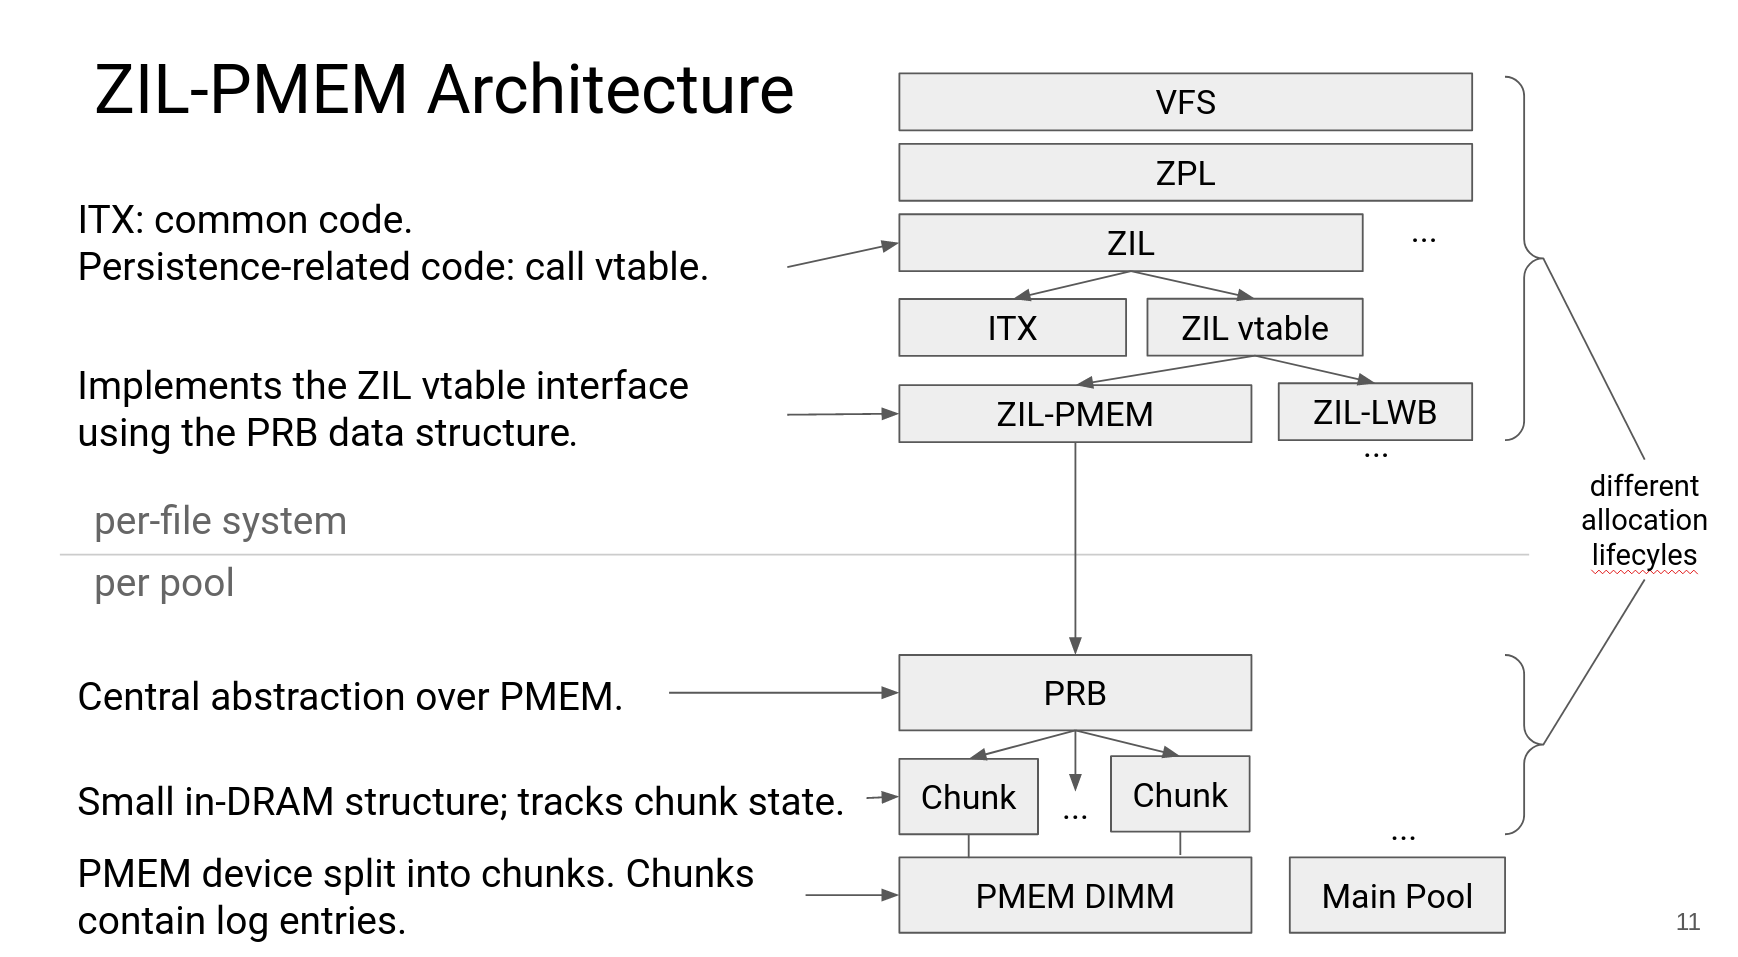
\includegraphics[height=20cm,width=\textwidth,keepaspectratio]{fig/zilpmem_architecture_overview}
    \caption{Overview of the system architecture as described in this section.}
\end{figure}~\todo{actual figure}

\section{PMEM-aware SPA \& VDEV layer}
In this section we describe how we add explicit support for PMEM to ZFS.
Our primary goal is to disable the SPA's metaslab allocation on PMEM SLOG devices so that ZIL-PMEM can use the allocatable space as PRB chunks.

We add a new boolean attribute \lstinline{is_dax} for \lstinline{disk} VDEVs in the zpool config format.
The attribute indicates whether the VDEV supports direct access through the DAX APIs.
Its value is determined by the \lstinline{zpool} command when creating or adding devices to a pool using \lstinline{libblkid}.
When opening a vdev marked \lstinline{is_dax}, the kernel module ensures that all of the block device's sectors are mappable as one contiguous range of kernel virtual address space.
Failure to establish this mapping fails the onlining process, leaving the vdev in state \lstinline{VDEV_STATE_CANT_OPEN}.
By default, this state prevents the pool from being imported.
If the VDEV is added as a log device, the import process allows the user to specify an override flag, causing the log to be dropped.
Note that the \lstinline{is_dax} feature applies to all VDEVs and is independent of ZIL-PMEM.
It merely records the fact that a VDEV is required to be directly accissble via the DAX APIs.

To disable metaslab allocation on PMEM SLOGs, we introduce a new allocation class called \lstinline{exempt}.
When adding a log device to the pool that is \lstinline{is_dax}, the \lstinline{zpool} command assigns it to the \lstinline{exempt} class instead of the \lstinline{log} class.
This alone is sufficient to prevent allocation from PMEM SLOGs because the \lstinline{exempt} allocation class by convention is never used.
The allocatable space on the device is thus never read or written through ZIO and available for use by ZIL-PMEM.
Note that reads and writes to VDEV labels\todo{need to explain this? short analogy: partition header} are located outside of the allocatable space.
Updates to VDEV labels continue to be made using block device IO (\lstinline{zio_read_phys} and \lstinline{zio_write_phys}).

\begin{figure}[h]
    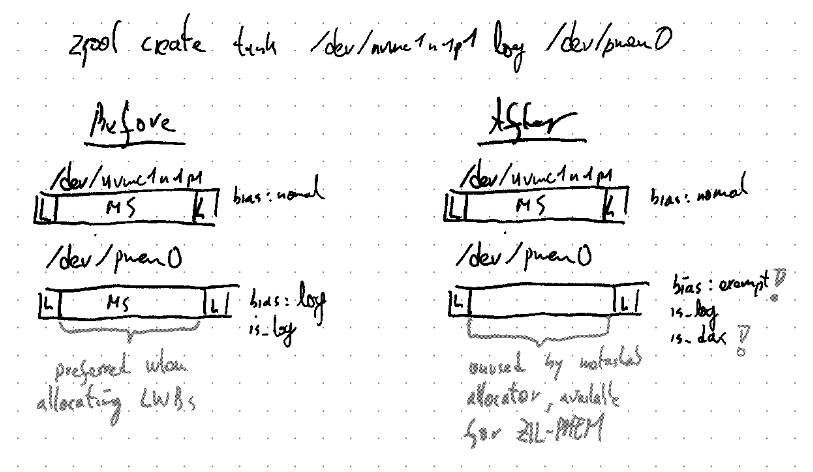
\includegraphics[width=\textwidth]{fig/pmem_aware_vdev_layer_before_after}
    \caption{
        Comparison of the zpool layout before and after the addition of the \lstinline{is_dax} vdev attribute and the \lstinline{exempt} allocation class for PMEM SLOGs.
    }
\end{figure}

\section{ZIL kinds}
Coexistence with the existing ZIL and preservation of ZFS's crash consistency guarantees are two hard requirements for ZIL-PMEM (see Section~\ref{sec:requirements}).
Our solution to both of these problems is to re-architect ZFS to support different persistence strategies for the ZIL while sharing code and data structures that ultimately define crash consistency semantics.
In order to make the integration of ZIL-PMEM seamless to the end user (goal: simple administration), the persistence strategy is the same for all datasets in a pool.
The variable that determines the pool's persistence strategy is its \textit{ZIL kind}.
The following sub-sections present how we refactored ZFS to support ZIL kinds.
The existing ZIL which uses LWBs for persistence becomes the first ZIL kind called ZIL-LWB.
Note that some listings in this section already mention ZIL-PMEM to illustrate why ZIL kinds are necessary to integrate ZIL-PMEM.
However, in our implementation, all refactoring steps presented in this section are separate commits that precede the introduction of the ZIL-PMEM ZIL kind.

\subsection{On-Disk State}\label{sec:di:zil_header}
As described in Section~\ref{openzfs:the_zil_on_disk_format} the ZIL(-LWB) keeps its persistent state in the per-dataset ZIL header and the LWB chain.
For ZIL kinds, we change the ZIL header to be a tagged union that uses the new \lstinline{zh_kind_t} enum as a discriminant.
The existing ZIL-LWB header fields are moved into the \lstinline{zil_header_lwb_t} type.
ZIL-PMEM's ZIL header, which we describe in Section~\ref{sec:zilpmem}, is the second type in that union.
We maintain the same size as the original \lstinline{zil_header_t} by using one 64 bit word of padding, thereby simplifying the on-disk format migration.
Figure~\ref{lst:zil_header_before_and_after} shows the relevant C structures before and after the changes described in this paragraph.

\begin{figure}[h]
\begin{subfigure}[t]{0.45\textwidth}
\begin{lstlisting}
typedef struct zil_header {
  uint64_t zh_claim_txg;
  uint64_t zh_replay_seq;
  blkptr_t zh_log;
  uint64_t zh_claim_blk_seq;
  uint64_t zh_flags;
  uint64_t zh_claim_lr_seq;
  uint64_t zh_pad[3];
} zil_header_t;
\end{lstlisting}
\end{subfigure}
\hfill
\begin{subfigure}[t]{0.5\textwidth}
\begin{lstlisting}
typedef enum {
    ZIL_KIND_UNINIT,
    ZIL_KIND_LWB,
    ZIL_KIND_PMEM,
    ZIL_KIND_COUNT
} zh_kind_t;

typedef
struct zil_header_lwb {
  /* fields of zil_header_t,
   * without zh_pad */
} zil_header_pmem_t;

typedef
struct zil_header_pmem {
  /* introduced later */
} zil_header_pmem_t;

typedef
struct zil_header {
  uint64_t zh_kind;
  union {
    zil_header_lwb_t  zh_lwb;
    zil_header_pmem_t zh_pmem;
  } zh_data;
  uint64_t zh_pad[2];
} zil_header_t;
\end{lstlisting}
\end{subfigure}
\caption{The ZIL header structs (in DRAM and on disk) before and after the introduction of ZIL kinds.}
\label{lst:zil_header_before_and_after}
\end{figure}

\subsection{Runtime State}\label{sec:zil_kinds:runtime}
As described in Section~\ref{openzfs:the_zil_api}, the ZIL(-LWB) runtime state is kept in the per-dataset object \lstinline{zilog_t}.
\lstinline{zilog_t} tracks the in-memory representation of log records (ITXs) in the \lstinline{itxg} struct until they become obsolete due to txg sync or need to be written to stable storage by \lstinline{zil_commit}.
\lstinline{zil_commit} drains the ITXs into the \textit{commit list}.
It proceeds by packing the ITXs on the commit list into LWBs which it writes to disk as a chain linked by ZFS block pointers.

We observe the following properties of the code that handles ITXs and \lstinline{itxgs}:
\begin{itemize}[noitemsep]
    \item It defines the framework for ZFS's crash consistency semantics.
          Whereas ZPL and ZVOL code fill the body of the log records, the organization by \lstinline{itxgs} and the code that assembles the commit list constraints what can be expressed as ZIL records.
    \item ITXs and even the commit list are independent of the LWB chain that is ultimately written to disk.
          The commit list merely defines the set of ZIL records that need to be persisted before \lstinline{zil_commit} can return, and in what order these log records must be replayed.
    \item The interface between the ITX- and LWB-related code is limited to the \textit{commit list} and its contents.
          Whereas the ITXs are not opaque to the LWB-related code (e.g. handling of \lstinline{WR_NEED_COPY}\todo{check that this was defined}), the responsibilities are cleanly separated.
\end{itemize}
Given these insights we refactor the ZIL implementation (\textit{zil.c}) as follows:
\begin{enumerate}[noitemsep]
    \item Move all non-ITX functions into a separate module \textit{zil\_lwb.c} and prefix them with \lstinline{zillwb_}.
          If the function was part of the public ZIL API, add a wrapper function with the original name to \textit{zil.c} that forwards the call to the \lstinline{zillwb_} function in \textit{zil\_lwb.c}.
    \item Virtualize calls to \lstinline{zillwb_} functions in \textit{zil.c}:
          \begin{itemize}
              \item Define a struct \lstinline{zil_vtable_t} that contains function pointers with the type signature of each of the \lstinline{zillwb_} functions called from \textit{zil.c}.
              \item Define \lstinline{zillwb_vtable} as an instance of \lstinline{zil_vtable_t} that uses \lstinline{zillwb_} functions as values for the respective function pointer members.
              \item Add a member \lstinline{zl_vtable} to \lstinline{zilog_t} that is pointer to a \lstinline{zil_vtable_t}.
              \item Replace all calls to \lstinline{zillwb_FN()} in \textit{zil.c} with indirect calls through the vtable, i.e., \lstinline{zilog->zl_vtable.FN()}.
          \end{itemize}
    \item Make non-ITX state private to \textit{zil\_lwb.c} by turning it into a subobject.
          \begin{itemize}
              \item Move the \lstinline{zilog_t} members that are only used by the functions in \textit{zil\_lwb.c} into a separate structure called \lstinline{zilog_lwb_t} that is private to \textit{zil\_lwb.c}.
              \item Embed \lstinline{zilog_t} as the first member in \lstinline{zilog_lwb_t}.
              \item Add member \lstinline{zlvt_alloc_size} to \lstinline{zl_vtable_t} that indicates the amount of memory to be allocated when allocating a \lstinline{zilog_t}.
              \item Add a \textit{downcast} step to the start of each \lstinline{zillwb_} function that casts the \lstinline{zilog_t} pointer into a \lstinline{zilog_lwb_t} pointer.
                The majority of functions can operate only on the \lstinline{zilog_lwb_t}-private state without accessing the embedded \lstinline{zilog_t}.
              \item Add constructor and destructor methods to the vtable that are called after allocating the \lstinline{zlvt_alloc_size}d \lstinline{zilog_t}.
                The \lstinline{zillwb_} constructor and destructors initialize and deinitialize the private members of \lstinline{zilog_lwb_t}.
          \end{itemize}
\end{enumerate}
The end result ist best described in the terminology of object-oriented programming:
\textbf{\lstinline{zilog_t} is an abstract baseclass} that implements the public ZIL interface as well as ITX-related functionality and defines abstract methods for persisting log records.
These abstract methods must be implemented by concrete subclasses.
\lstinline{zilog_lwb_t} is such a subclass that implements the LWB-based persistence strategy.
For ZIL-PMEM, the \lstinline{zilog_pmem_t} struct which we introduce in Section~\ref{sec:zilpmem} implements persistence directly to PMEM.
Which subclass is instantiated at runtime is determined by the \lstinline{zh_kind} field in the ZIL header (see Section~\ref{sec:di:zil_header} and Figure~\ref{lst:zil_header_before_and_after}).
Figures~\ref{fig:zilog_splitup_class_diagram} and \ref{fig:zilog_splitup_example_code} illustrate the changes described in this section.

\begin{figure}
\missingfigure[figheight=10cm]{}
\caption{\lstinline{zilog_t} before and after the introduction of ZIL kinds, visualized as a class diagram.}
\label{fig:zilog_splitup_class_diagram}
\end{figure}

\begin{figure}
\missingfigure[figheight=20cm]{}
\caption{The refactoring steps described in Section~\ref{sec:zil_kinds:runtime} by example of the \lstinline{zil_itx_assign()} and \lstinline{zil_commit()} APIs.}
\label{fig:zilog_splitup_example_code}
\end{figure}

\subsection{Changing ZIL Kinds}\label{sec:zil_kinds:change}
In the design overview (sec.~\ref{sec:design_overview}) we introduce ZIL kinds as a pool-scoped variable.
The pool's ZIL kind implicitly according to the following rule:
\begin{displayquote}
If the pool has exactly one SLOG and that SLOG is PMEM, the ZIL kind is ZIL-PMEM. Oterwise, it is ZIL-LWB.
\end{displayquote}
The rule is re-evaluated whenever a SLOG is added or removed, i.e., during pool creation and on \texttt{zpool add} and \texttt{zpool remove}.
The idea behind this approach is to keep administration simple --- a defining paradigm for ZFS:
ZIL-PMEM should be automatically activated if hardware and software support it and not be used otherwise.
%Note that the alternative significantly worsens\todo{that a word?} the user experience since they would need to configure the ZIL kind of each individual dataset, or rely on some auto-tuning mechanism.

To accomplish this behavior, the following steps must happen in the same transaction group as the SLOG addition or removal that triggered the change of ZIL kind:
\begin{enumerate}[noitemsep]
    \item Stop using the ZIL API and wait until all active calls to it have finished.
    \item Wait for all ZIL entries to become obsolete by waiting for the open txg to sync.
    \item \lstinline{zil_close()} and subsequently \lstinline{free()} the currently open \lstinline{zilog_t} instances.
    \item Replace all datasets' ZIL header with the new ZIL kind's default header.
        \lstinline{zh_kind} is now set to the new ZIL kind.
    \item Allocate the new \lstinline{zilog_t} instances and \lstinline{zil_open()} them.
        The allocation routine uses \lstinline{zh_kind} to select the (new) vtable, allocates \lstinline{zlvt_alloc_size} bytes for the new \lstinline{zilog_KIND_t} and runs the ZIL kind specific constructor.
\end{enumerate}
Due to time constraints we have \textbf{not yet implemented} this procedure.
As a stop-gap solution, we add a kernel module parameter \lstinline{zil_default_kind} that defines the ZIL kind that is used for the \lstinline{zh_kind} field in new dataset's ZIL headers.
There is no mechanism to change \lstinline{zh_kind} over the lifetime of a dataset.
It is possible to mix different ZIL kinds in the same pool by changing \lstinline{zil_default_kind} before creating a new dataset.
This works correctly but is undesirable from a usability perspective because we want ZIL kinds to be transparent to the user.
% DON'T point out that the design alternative is to have internal polymorphism within zilog_t. It's trivial to see from an implementor's perspective.

\subsection{ZIL-LWB Suspend \& Resume}\label{sec:zil_kinds:suspend_resume}
The ZIL API provides the \lstinline{zil_suspend} and \lstinline{zil_resume} functions.
\lstinline{zil_suspend} pauses all ZIL activity and ensures that all log entries are obsolete.
\lstinline{zil_resume} reverts the state to normal operation.
Compatibility code for versions of ZFS prior to the \textit{fast snapshots} feature must use them for snapshots.
For newer pool versions, the only consumer \lstinline{spa_reset_logs}: when removing a SLOG from the pool, the ZIL is temporarily suspended to ensure that the SLOG does not contain valid log entries.
Once the ZIL resumes and starts allocating LWBs, the metaslab allocator transparently uses other SLOGs or the main pool devices.

With regards to ZIL kinds, only the \lstinline{spa_reset_logs} use case is relevant since ZIL kinds require a more recent pool version than the \textit{fast snapshots} feature.
Our design for changing ZIL kinds (Section~\ref{sec:zil_kinds:change}) requires suspension of all ZIL activity and thus subsumes the ZIL-LWB specific \lstinline{zil_suspend} and \lstinline{zil_resume}.
However, the compatibility code for pools before \textit{fast snapshots} needs to be maintained in a way that does not depend on the ZIL kinds feature.
Due to time constraints, we were \textbf{unable to address suspend \& resume in our design}.
We expect that the solution will be highly dependent on implementation-level constraints.

\subsection{ZIL Traversal \& ZDB}\label{sec:zil_kinds:traversal}
Whereas ZIL replay is abstracted away by the \lstinline{zilog_t} refactoring, there are several cases where the raw ZIL-LWB chain is traversed directly using the \lstinline{zil_parse} function.
\lstinline{zil_parse} exposes several ZIL-LWB implementation details to its callers such as the concept of LWBs and blockpointers.
This is problematic for ZIL kinds because not every conceivable ZIL kind uses these concepts; ZIL-PMEM being the obvious example.
We investigate all users of the ZIL traversal code and come to the conclusion that there is no need for a generalized interface that every ZIL kind needs to implement.
The basis for this decision is a manual analysis of \lstinline{zil_parse}'s callers.
\begin{description}[noitemsep]
    \item[dmu\_traverse] This module implements a callback-based traversal of the zpool's data structures.
    It is used to implement many ZFS features, e.g., \textit{zfs send}.
    If a dataset is traversed that is a head dataset (i.e., not a snapshot) and its LWB chain has been claimed, the LWBs are included in the traversal.
    \item[dsl\_scan\_zil] During a \textit{zpool scrub} (data integrity check of the entire pool), this function traverses claimed LWB chains.
    \item[spa\_load\_verify] During pool import this function uses \textit{dmu\_traverse} to traverse data structures updated in the last synced transaction groups.
    \item[zdb\_il.c] The \textit{ZFS debugger} interprets the ZIL header of head datasets, traverses their LWB chain, and dumps its contents to stdout.
\end{description}
Most consumers of \textit{dmu\_traverse} operate on snapshots, not head datasets, and therefore do not trigger ZIL chain traversal.
The \textit{dsl\_scan} and \textit{spa\_load} code does not actually use the ZIL data because the data integrity checks are implemented transparently in the ZIO read pipeline.
One compatibility code path (\lstinline{old_synchronous_dataset_destroy}) uses ZIL traversal to free the ZIL blocks, but can be replaced with a more recent API (\lstinline{zil_destroy_sync}).
\textit{zdb} is an exception since its whole purpose is to interpret the ZIL chain for debugging purposes.

Given this analysis we implement the following change as a precursor to the refactoring of \lstinline{zilog_t} described in Section~\ref{sec:zil_kinds:runtime}.
We change the \lstinline{zil_parse} API to work directly on a \lstinline{zil_header_lwb_t*} instead of \lstinline{zilog_t}.
We also rename the function to \lstinline{zillwb_parse_phys} to reflect the fact that it is specific to ZIL-LWB and does not affect runtime state.
Finally, we change the \textit{dmu\_traverse} API so that callers must be explicit about ZIL-LWB traversal which we believe will ease maintainability in the future.
We \lstinline{zil_destroy_sync} in \lstinline{old_synchronous_dataset_destroy}, leaving \lstinline{spa_load_verify} as the only consumer of the \textit{dmu\_traverse} API that needs to traverse ZIL-LWB chain.


\subsection{ZIL-LWB-Specific Callbacks}\label{sec:zil_kinds:callbacks}
There are several callbacks from modules outside of ZIL-LWB.
Since these callbacks are made through static function calls --- not function pointers --- they are part of the ZIL's public API and need to be considered for our ZIL kind refactoring.
However, none of them are necessary for ZIL-PMEM.
Therefore, we prefix the callback functions with \lstinline{zillwb_}, move them to \textit{zil\_lwb.c} and ignore them in the remainder of this thesis.
For maintainability, future work should replace these statically dispatched callbacks with dynamic callbacks through function pointers to increase decoupling.
We list the APIs in question so that this issue can be addressed in future work:
\begin{description}
    \item[zil\_lwb\_add\_txg] Necessary to keep the in-DRAM representation of an LWB alive when writing \lstinline{WR_INDIRECT} blocks.
    \textbf{Note}: we can only afford to ignore this function because ZIL-PMEM does not support \lstinline{WR_INDIRECT} blocks.
    \item[zil\_lwb\_add\_block] Necessary for an optimization that minimizes the amount of flush commands that are sent to the SLOG device.
    \item[zil\_bp\_tree\_add] During a ZIL traversal with \lstinline{zil_parse}, this API was used to avoid doing operation more than once for a given blockpointer.
        It is an implementation detail of ZIL-LWB that is only a public ZIL API because it is used by \textit{zdb}'s ZIL traversal code.
\end{description}

\subsection{Considered Alternatives}
The general concept of ZIL kinds and the vtable-based implementation add complexity to the ZIL code.
In this section we discuss the alternatives that we considered for supporting multilpe ZIL implementations at runtime.

\textbf{Alternative \#1}: We considered moving the dispatch into ZIL kind specific code one API layer up so that \lstinline{zilog_t} and ITX would be completely specific to ZIL-LWB.
The API layer that we considered are the \lstinline{zfs_log_OP} and \lstinline{zvol_log_OP} helper functions which create and assign ITXs for ZPL and ZVOL operations.
The sequence diagram in Figure~\ref{fig:zfs_log_write_sequence_diagram} provides an example of how a \lstinline{write} system call uses this API.
Declaring this API layer the interface for ZIL kinds would allow ZIL implementations to chose freely how they want to represent log records in DRAM and on stable storage.
This additional freedom could be used by future ZIL kinds to implement a different log structure with better scalability or more fine-grained crash consistency guarantees.
For example, an earlier design for ZIL-PMEM used a graph-based log structure where log entries for a file in the same dataset could be written in parallel.
However, the additional freedom also has significant drawbacks that ultimately led us to the design presented in the previous subsections:
\begin{enumerate}[noitemsep]
    \item The \lstinline{zfs_log_OP} family of functions only addresses the ZIL write path.
        There are no equivalent abstractions that wrap the \lstinline{zilog_t} APIs for ZIL replay or traversal.
        In order to have a single clean abstraction at the level of \lstinline{zfs_log_OP}, it would be necessary to extend this API so that \lstinline{zilog_t} could be hidden as an implementation detail of ZIL-LWB.
        We were not confident in our ability to design this API extension without the risk of introducing a leaky abstraction.
    \item ZIL kind specific functions for logging would also require ZIL kind specific replay functions.
        In ZIL-LWB this is a non-trivial amount of code.
        ZIL kinds such as ZIL-LWB that only implement a different persistence strategy would have to duplicate this code, pointlessly increasing maintenance cost.
    \item We find it undesirable to allow ZIL-kinds to implement different crash consistency guarantees, in particular if ZIL kinds switch automatically depending on SLOG hardware (see Section~\ref{sec:zil_kinds:change}).
        Centralizing the ITX code and forcing every ZIL kind to fit into the ITX model is the best way to ensure that crash consistency guarantees are the same across ZIL kinds.
\end{enumerate}

\begin{figure}
    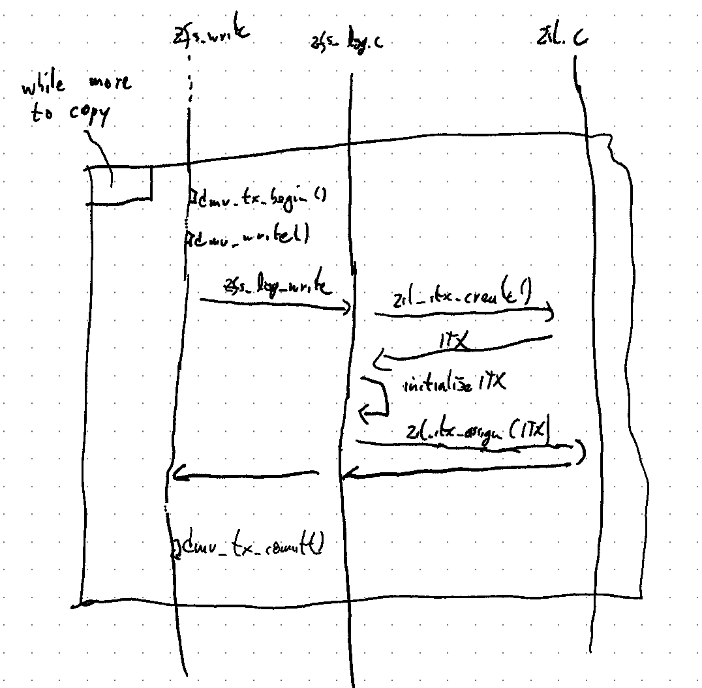
\includegraphics[height=8cm]{fig/zfs_log_write_sequence_diagram}
    \label{fig:zfs_log_write_sequence_diagram}
    \caption{Sequence diagram of the APIs involved in creating the ITXs for a \lstinline{write} system call.}
\end{figure}

\textbf{Alternative \#2}: Since we identified the ZIO pipeline as the main source of latency\todo{ref chapter} in ZIL-LWB, we considered sharing LWBs as a concept between all ZIL kinds.
In that scenario, the ZIL kinds would merely be an alternative to the ZIO pipeline.
A prototype that adopts this approach has been presented at the OpenZFS 2020 Developer summit by \citeauthor{openzfsZILPerformanceImprovements2020}, targeting NVMe drives \cite{openzfsZILPerformanceImprovements2020}
We found this layer of the ZFS software stack to be too restrictive for ZIL-PMEM:
\begin{enumerate}
    \item The timeout mechanism\todo{ref} for packing multiple entries into a single LWB would add unnecessary latency overhead.
        This is in conflict with one of our requirements (see Section~\ref{sec:requirements}).
    \item This notion is shared by the database community which has deemed group commit schemes --- such as LWB timeout --- unfit for PMEM (see Section~\ref{relw:groupcommit}).
    \item The PRB's feature to log entries for the same dataset in parallel\todo{ref} would not have been possible if ZIL-PMEM would be constrained to LWBs.
        Our ITXG bypass for ZVOLs (see Section~\ref{sec:itxg_bypass}) shows how we can use this PRB feature to increase scalability\todo{check,ref} without compromising on crash consistency guarantees.
\end{enumerate}

\subsection{Summary}
We believe that our design for ZIL kinds introduces ZIL kind specific behavior at the layer that allows for sufficient flexibility in the implementation without adding unnecessary abstractions and maintenance burden.
The interface defined by the vtable is a clean abstraction although some design questions (see \ref{sec:zil_kinds:change} and \ref{sec:zil_kinds:suspend_resume}) as well as some LWB-specific APIs (see \ref{sec:zil_kinds:traversal} and \ref{sec:zil_kinds:callbacks}) remain.
The state of each \lstinline{zilog_KIND_t} is truly private do the ZIL kind's implementation.
Neither ZIL-LWB nor ZIL-PMEM access the ITX-related state in the embedded \lstinline{zilog_t} directly, but only\todo{"sondern"?} through the \lstinline{zilog_t} method that computes the commit list.
If requirements change in the future, the design alternatives presented in the previous section should be considered.

\section{PRB/HDL: A generic logical WAL for a zpool}
In this section we describe the PRB/HDL data structure in detail.

% PRB log entries consist of an opaque variable-sized body and a plain fixed-size header.
% A log entry is always written to exactly one chunk's PMEM segment.
% The segment is organized as a contiguous append-only sequence of entries that is terminated by an invalid header.
% %Starting with the first entry's header at offset zero, the sequence can be traversed using length information stored in the headers.
% If a chunk's remaining space is too small to fit an entry, the writer puts the chunk on a "full list" where it sits until all of the full chunk's entries are obsoleted by txg sync.
% Once all entries are obsolete, the full chunk is moved to the "free list" for reuse by a writer.
% Each entry header stores sufficient metadata to attribute entries to a dataset, detect data corruption and missing entries, and order entries for replay based on sequence numbers.
% The physical location of entries in PMEM is irrelevant for replay.
% Instead, replay traverses each chunk's entries, filters them for the given dataset and constructs a replay sequence in DRAM using the ordering information stored in the entry headers.

\section{ZIL-PMEM}
In this section we describe how we use PRB/HDL to implement ZIL-PMEM as a new ZIL kind.

\section{ITXG Bypass For ZVOL}
In this section we describe a performance optimization for ZIL-PMEM that allows for parallel log writes to a single ZVOL.

\chapter{Evaluation}\label{ch:eval}
\section{Correctness}
We evaluate the correctness of our work through unit and integration tests.
\subsection{PRB}
\subsection{ZIL-PMEM}
\section{Performance}
We evaluate the performance of ZIL-PMEM with a variety I/O benchmarks.
\subsection{Write Performance}
\subsubsection{4k Random Sync Writes}
\subsubsection{Application Benchmarks}
\subsection{Replay Performance}

\chapter{Related Work}

\backmatter

\chapter{Appendix}\label{ch:appendix}

\cleardoublepage
\phantomsection
\addcontentsline{toc}{chapter}{Bibliography}
\emergencystretch=1em
\printbibliography

\end{document}
